% Copyright 2004 by Till Tantau <tantau@users.sourceforge.net>.
%
% In principle, this file can be redistributed and/or modified under
% the terms of the GNU Public License, version 2.
%
% However, this file is supposed to be a template to be modified
% for your own needs. For this reason, if you use this file as a
% template and not specifically distribute it as part of a another
% package/program, I grant the extra permission to freely copy and
% modify this file as you see fit and even to delete this copyright
% notice. 
\documentclass{beamer}

% There are many different themes available for Beamer. A comprehensive
% list with examples is given here:
% http://deic.uab.es/~iblanes/beamer_gallery/index_by_theme.html
% You can uncomment the themes below if you would like to use a different
% one:
%\usetheme{AnnArbor}
%\usetheme{Antibes}
%\usetheme{Bergen}
%\usetheme{Berkeley}
%\usetheme{Berlin}
%\usetheme{Boadilla}
%\usetheme{boxes}
%\usetheme{CambridgeUS}
%\usetheme{Copenhagen}
%\usetheme{Darmstadt}
%\usetheme{default}
%\usetheme{Frankfurt}
\usepackage{multimedia}
\usetheme{Malmoe}
\definecolor{UniBlue}{RGB}{52,38,206}
\newcommand{\wl}[2]{\href{#1}{\textcolor{UniBlue}{#2}}}
%\definecolor{UniGray}{RGB}{20,40,40}
%\definecolor{UniGray}{RGB}{28,33,43}
\definecolor{UniGray}{RGB}{9,21,64}
%\definecolor{UniGray}{RGB}{13,124,82}
\definecolor{UniGreen}{RGB}{0,177,89}
\definecolor{LightGray}{RGB}{201,201,201}
% \setbeamercolor{title}{fg=UniBlue}
% \setbeamercolor{frametitle}{fg=UniBlue}
% \setbeamercolor{structure}{fg=UniBlue}
\usecolortheme[named=UniBlue]{structure}
\setbeamercolor{section in head/foot}{fg=white, bg=UniGray}
\setbeamertemplate{footline}%{miniframes theme}
  {%
    \begin{beamercolorbox}[colsep=1.5pt]{upper separation line foot}
    \end{beamercolorbox}
    \begin{beamercolorbox}[ht=2.5ex,dp=1.125ex,%
      leftskip=.3cm,rightskip=.3cm plus1fil]{author in head/foot}%
      \leavevmode{\usebeamerfont{author in head/foot}\insertshortauthor}%
      \hfill%
      {\usebeamerfont{institute in head/foot}\usebeamercolor[fg]{institute in head/foot}\insertshortinstitute}%
    \end{beamercolorbox}%
    \begin{beamercolorbox}[ht=2.5ex,dp=1.125ex,%
      leftskip=.3cm,rightskip=.3cm plus1fil]{title in head/foot}%
      {\usebeamerfont{title in head/foot}\insertshorttitle} \hfill     \insertframenumber%
    \end{beamercolorbox}%
    \begin{beamercolorbox}[colsep=1.5pt]{lower separation line foot}
    \end{beamercolorbox}
  }

%footnote size
%\usefonttheme[stillsansseriflarge]{serif}
%\renewcommand\labelenumi{(\theenumi)}
\setbeamertemplate{bibliography entry title}{}
\setbeamertemplate{bibliography entry location}{}
\setbeamertemplate{bibliography entry note}{}
\usepackage[font=scriptsize,labelfont=bf]{caption}
\usepackage{dirtree}
\usepackage{textcomp}
\usepackage{multirow}
\usepackage{tabularx}
\usepackage{soul}
% \setbeamercolor{frametitle}{fg=brown}
%\usetheme{Hannover}
%\usetheme{Ilmenau}
%\usetheme{JuanLesPins}
%\usetheme{Luebeck}
%\usetheme{Madrid}
%\usetheme{Malmoe}
%\usetheme{Marburg}
%\usetheme{Montpellier}
%\usetheme{PaloAlto}
%\usetheme{Pittsburgh}
%\usetheme{Rochester}
%\usetheme{Singapore}
%\usetheme{Szeged}
%\usetheme{Warsaw}

\title{A Developer's Life after University}
\subtitle{Life and pre-career of a software developer in University}
% A subtitle is optional and this may be deleted
% \subtitle{Optional Subtitle}


% - Give the names in the same order as the appear in the paper.
% - Use the \inst{?} command only if the authors have different
%   affiliation.

\institute[DevClub] % (optional, but mostly needed)
{
  \inst{}
  Come, Code, and Make IT happen!
  \and
  \inst{}

\includegraphics[width=3cm]{images/devclub.jpg}}
  \author{Mustafa Ehsan Alokozay}
% - Use the \inst command only if there are several affiliations.
% - Keep it simple, no one is interested in your street address.

\date{\tiny{\today}}
% - Either use conference name or its abbreviation.
% - Not really informative to the audience, more for people (including
%   yourself) who are reading the slides online

\subject{Technical Presentation}
% This is only inserted into the PDF information catalog. Can be left
% out. 

% If you have a file called "university-logo-filename.xxx", where xxx
% is a graphic format that can be processed by latex or pdflatex,
% resp., then you can add a logo as follows:

% \pgfdeclareimage[height=0.4cm]{university-logo}{tlulogo}
% \logo{\pgfuseimage{university-logo}}

% Delete this, if you do not want the table of contents to pop up at
% the beginning of each subsection:
% \AtBeginSubsection[]
% {
%   \begin{frame}<beamer>{Agenda}
%     \tableofcontents[currentsection,currentsubsection]
%   \end{frame}
% }

% Let's get started
\begin{document}

\begin{frame}
  \titlepage
\end{frame}

\begin{frame}{Table of Contents}
  \tableofcontents
  % You might wish to add the option [pausesections]
\end{frame}

% Section and subsections will appear in the presentation overview
% and table of contents.

\section{Introduction}
\subsection{Who am I?}

\begin{frame}{Who am I?}
	\begin{itemize}
		\item I am Mustafa Ehsan
		\item A software developer at Netlinks
		\item Open source contributor and lover
	\end{itemize}		
\end{frame}

% ########################################################################

\section{University Days}
\subsection{Your Boring Black Screen}

\begin{frame}{Don't get upset with your black screen}
	\begin{itemize}
		\item Loops, blocks, assignments, if...else, black screens will always be there, master them.
		\item From building a simple calculator to writing code for NASA's spaceships your loops and if, elses will be always be with you.
	\end{itemize}
	\centering
	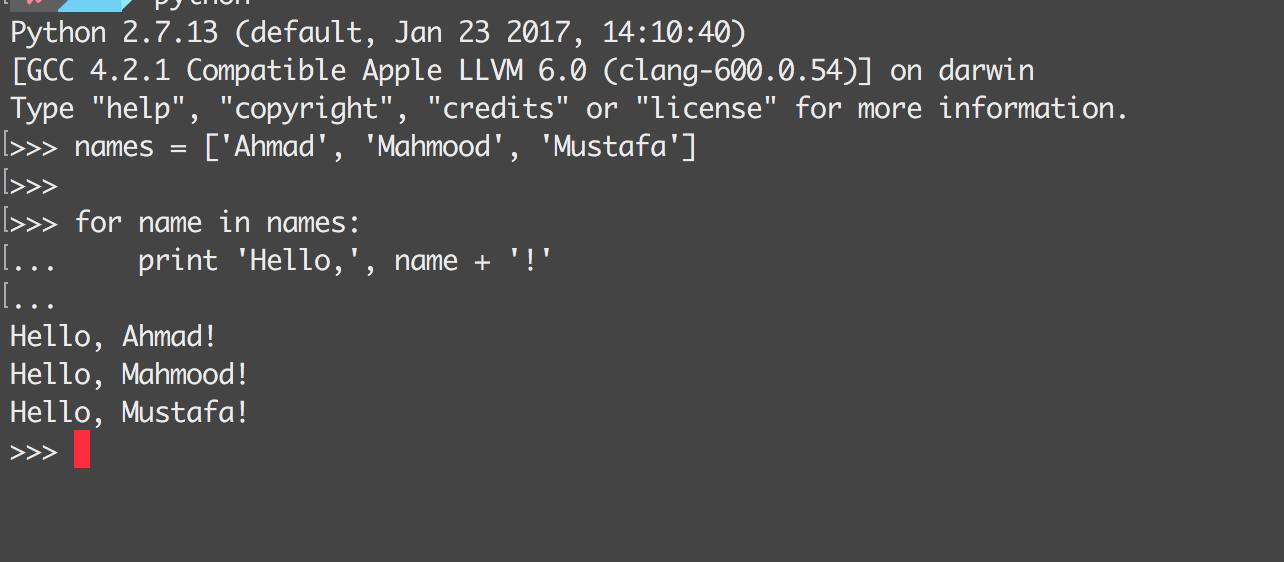
\includegraphics[width=10cm]{images/black_screen.png}
\end{frame}


\subsection{Data Structures and Algorithms}
\begin{frame}{What good is there in data structures/algorithms for you?}
	\begin{itemize}
		\item Is there any good in it?
		\item Logic and decision making
		\item Big companies interviews
		\item Reducing complexity
	\end{itemize}
\end{frame}

\section{Personality Tips}
\subsection{Things to Know}

\begin{frame}{Things to Know}
	\begin{itemize}
		\item If you cannot answer your "why?", don't go forward
		\item Sometimes, don't listen to your family; ask them why?
		\item If you love it, you will get it
		\item Don't let university kill you
		\item Go out and enjoy your time
	\end{itemize}
\end{frame}

\subsection{Things to do}

\begin{frame}{Things to do}
	\begin{itemize}
		\item Build small things, but usable things
		\item Start automation from today, start with ugly scripts
		\item Reinvent the wheel as much as you can
	\end{itemize}
\end{frame}

\section{Your Career}
\subsection{Pre-Career Tips}
\begin{frame}{Pre-Career Tips}
	\begin{itemize}
		\item Be a specialist, be a generalist
		\item Have something to show
		\item Be fair and realistic about your incomes
		\item Make decisions with your current state in mind
		\item Ge involved in open source (long term tip)
	\end{itemize}
\end{frame}

\subsection{Career paths in Software}
\begin{frame}{Career paths in Software}
	Below is some career paths that someone can follow in Afghanistan:
	\begin{itemize}
		\item Working for a vendor as a developer
		\item Starting a company (ahh, this is tough!)
		\item Working from home
		\item Remote jobs
	\end{itemize}
\end{frame}

\subsection{Open Source Involvement}
\begin{frame}{Open Source Involvement}
	\begin{itemize}
		\item You will learn, a whole lot
		\item You will be peer with industry's bests
		\item Learning the best possible practices in a technology
		\item It can even help you make a lot of money
		\item It can help you start a business out of it
	\end{itemize}
\end{frame}

\section{Some Success Stories}
\subsection{Sher Shah Rahim's Story}
\begin{frame}{Sher Shah Rahim's Story}
	A friend of mine who couldn’t speak English wanted to type Pashto which wasn’t possible back then with the built-in or third-party keyboards. I moved forward and developed one, today I have over 130,000 active users for my keyboard and Afghan Calendar. \newline
	
	It doesn’t only benefit others but it also gives me something in return. Just by placing Google Ads in the apps and not spending a penny, I make about \$500 a month.  
\end{frame}

\begin{frame}{Sher Shah's Advice}
	Do not choose computer science for money or for fame or for family, choose it only if you love it and only then you will shine.
\end{frame}

\subsection{Mustafa Wahrez's Story}
\begin{frame}{Mustafa Wahrez's Story}
	Graduated from Kabul University, he built a School Management System as his final year project and now he has turned it into a business. \wl{http://www.wsmis.com/}{WSMIS} is used among 49 schools in 12 different provinces of Afghanistan.
\end{frame}

\section{Open Source Career}
\subsection{Taylor Otwell}
\begin{frame}{Taylor Otwell}
	\centering
	
\includegraphics[width=3cm]{images/taylor.jpg}

	\begin{itemize}
		\item Creator of Laravel
		\item Forge, Envoyer, Spark
		\item Making about \$1.5M USD per month
	\end{itemize}
\end{frame}

\subsection{Mohamed Said}
\begin{frame}{Mohamed Said}
	\centering
	
\includegraphics[width=3cm]{images/said.jpg}

	\begin{itemize}
		\item A PHP developer from Egypt
		\item Started working on open source about 1.5 year ago
		\item Recently hired as Laravel's first employee
	\end{itemize}
\end{frame}

\section{Suggested Resources}
\subsection{CS50 from Harvard University}
\begin{frame}{CS50 from Harvard University}
	\begin{itemize}
		\item Harvard University's publicly available CS course
		\item Course website: \wl{https://cs50.harvard.edu/}{https://cs50.harvard.edu/}
		\item Spring and Fall semesters
	\end{itemize}
\end{frame}

\subsection{Code.org}
\begin{frame}{Code.org}
	\begin{itemize}
		\item An organization which aims to bring computer science to schools and to non-programmers
		\item Website: \wl{https://code.org/}{https://code.org/}
	\end{itemize}
\end{frame}






























% You can reveal the parts of a slide one at a time
% with the \pause command:

%\begin{frame}{Research Domain}
%\dirtree{% This % is required
%.1 e-Government. 
%.2 \textcolor{LightGray}{\small Models}.
%.3 \textcolor{LightGray}{\small {G2C, G2B, G2G, G2E, G2N}}. 
%.2 \textcolor{LightGray}{\small {Challenges, Opportunities, Barriers}}.
%.2 \textcolor{LightGray}{\small {Trust, User's Acceptance, Risks}}.
%.2 Frameworks (Architecture).
%.3 \textcolor{LightGray}{\small {Strategic}}.
%.3 Technical.
%.4 \textcolor{LightGray}{\small {Interoperability}}.
%.4 \textcolor{LightGray}{\small {Cloud-Based}}.
%.4 Key-Enablers or Building Block.
%.5 eIdentification, eSignature, eDocuments.
%.5 Characteristics/Features, Ranking.
%}
%
%\end{frame}






\section*{Questions}
\begin{frame}{}
\centering
\textcolor{UniBlue}{\Large \textbf{Thank you!}} \\
Questions?

{\color{UniBlue} \rule{\linewidth}{0.2mm} }
\wl{mailto:mehsan@devclub.af}{mehsan@devclub.af}\\
\wl{www.devclub.af}{www.devclub.af}\\
Twitter: \wl{https://twitter.com/mustafaaloko}{@mustafaaloko}\\
GitHub: \wl{https://github.com/mustafaaloko}{@mustafaaloko}\\
\end{frame}

\end{document}


